\chapter{Légzés}

\keywords{\emph{ānāpānasati} módszer és testtartás röviden}

\noindent A lélegzet érzéseit figyeljük a testben, ez az éber figyelem
az elmét egy stabil tárgy köré gyűjti össze. A test érzései jól
észrevehetőek miközben be- és ki lélegzünk. Ez a módszer
\emph{ānāpānasati} néven ismert, vagyis éberség a lélegzetre.

Miért annyira fárasztó a sok gondolkodás? Az elme egyik gondolattól a
másikig ugrál, de nem tudjuk hova megyünk és így sosem érkezünk meg. A
nyugtalan vágy kimerítő. Az érzéki visszafogottság összegyűjti az
energiát és irányítja azt, nem engedi szétfolyni minden irányba. A
figyelmet egy semleges, egyenletes érzésre irányítjuk, ami lelassítja a
gondolkodó elmét.

Ülhetsz a padlón, a szőnyeget és egy párnát használva, vagy egy széken
is. A padlón ülve, találj olyan helyzetet, ami nem erőlteti túl az
inakat vagy térdeket.

Széken ülve, húzódj előre az ülésen, hogy a hátad ne támaszd a
háttámlának. A támasz befolyásolja a gerinc alakját, és a légzés
ritmusát.

Tartsd a fejet egyensúlyban úgy, hogy a súlya ne húzzon előre. Mivel
gyakran széken ülünk, szokásunk a fejet előre tartani, ami a hátizmokban
hoz létre feszültséget. A fejet egy kicsit hátrahúzva érezzük, hogy
ellazulnak a hátizmok. Jó, ha az áll kissé behúzódik, de nem kell
erőltetni.

\clearpage
\thispagestyle{empty}\mbox{}
\contentFullBleed{%
\centering
\null\vfill

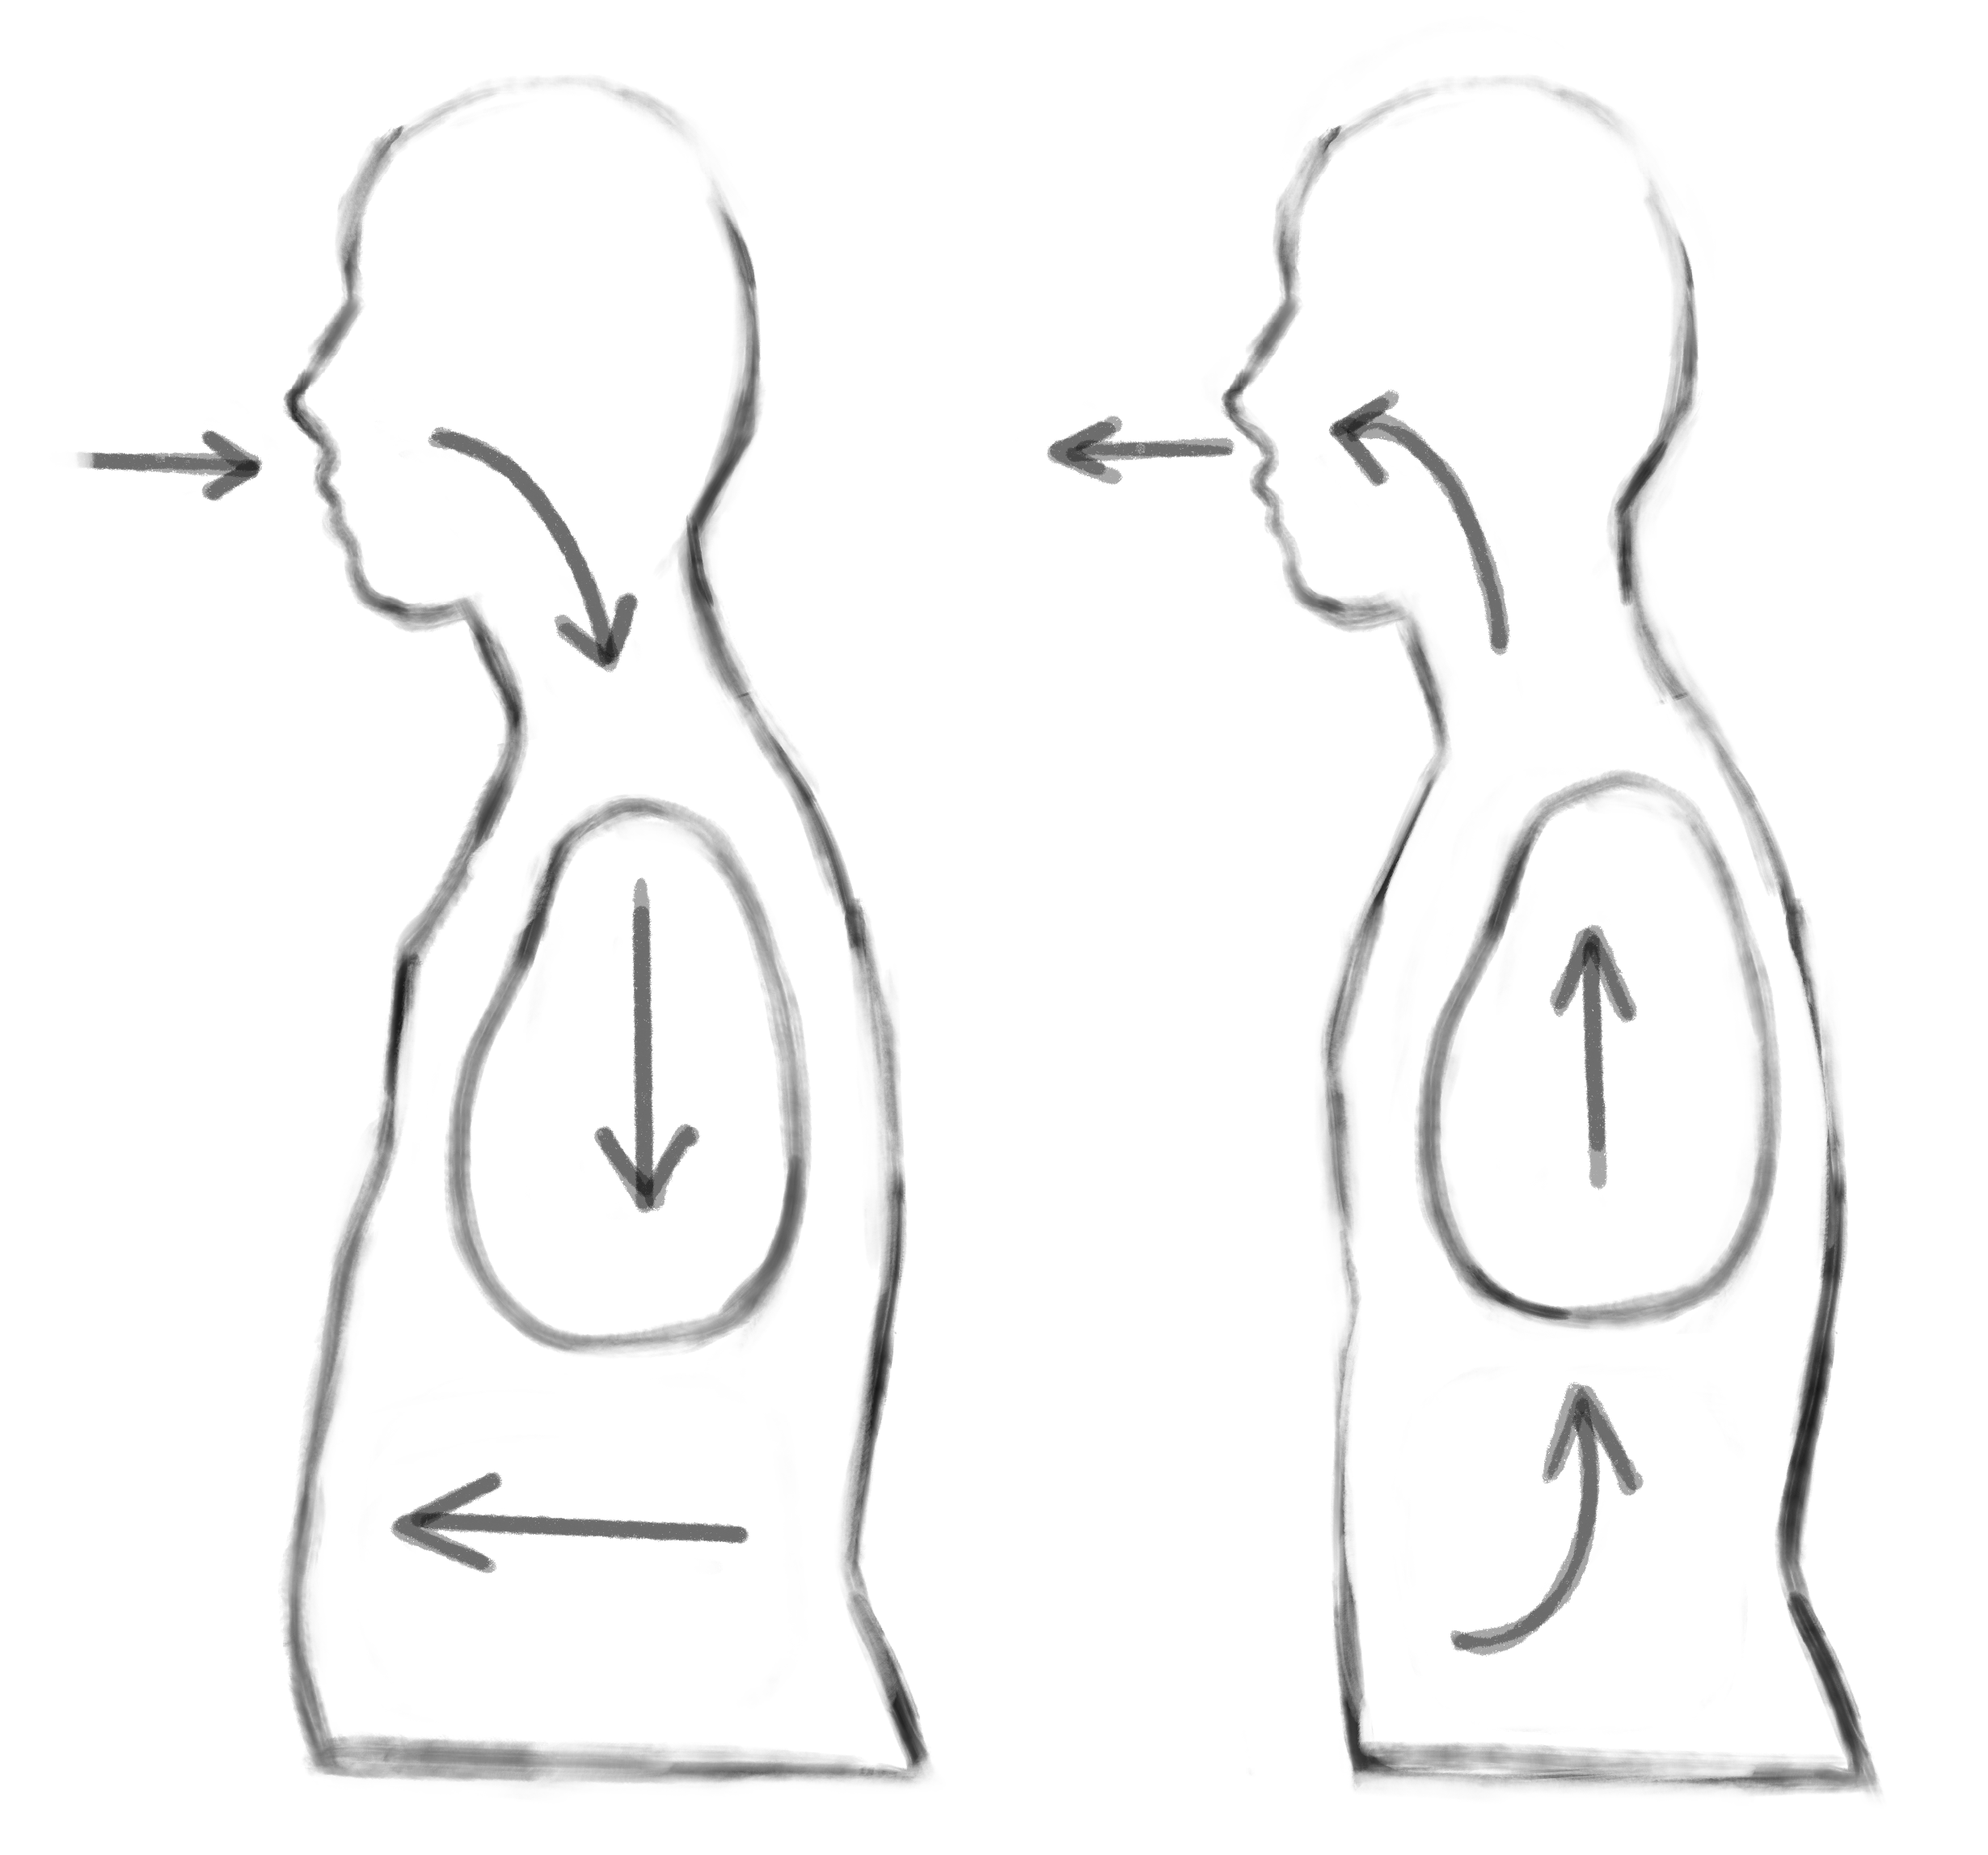
\includegraphics[width=\linewidth-20mm]{breathing.png}

\illustration{Légzés Technika}%
\label{illus-breathing}%

\vfill\null
}
\clearpage

Ülj egyenesen, kiegyensúlyozott testtartásban, a vállakat ellazítva. Jó
tartással a légzés könnyű és egyenletes.

A test csontjai úgy ülnek egymáson mint egy kövekből rakott torony. A
csípő-csont a párnán nyugszik, a gerinc a csípőn, a gerinc-korongok
egymásra rakva, a tetején a koponya, az egész torony középvonala
óvatosan egyensúlyban tartva.

Ha óvatosan ki van egyensúlyozva, és a súlypont középen van, nem
szükséges az izmok erejével húzni-vonni a testet, hogy megtartsuk. A
gravitáció elég ahhoz, egyenesben tartsa.

Belégzéskor, a hideg levegőt először az orrhegynél érezzük. Hagyd, hogy
a hasizmok irányítsák a levegővételt, ahelyett, hogy a mellkast tágítva
növelnéd a térfogatot. A levegő áthalad a tüdőn, és a has kitágul; ez a
légzési módszer csökkenti a szívritmust és feszültséget. Ellazítjuk az
izmokat, és a levegő az orron át távozik. Nem kell ezt precízen
irányítanunk, elegendő finoman utalni erre a ritmusra. A test magától is
tudja hogyan kell lélegezni, visszalépünk és figyelünk, mintha
hullámokat néznénk ahogy besodródnak a partra, majd visszahúzódnak.

Nem kell megmondanunk magunknak mit gondoljunk és mit érezzünk. Ha
tiszta gondolatokat akarunk, legjobb először csendben lenni és figyelni.
Csendben ülünk és pihenünk egy kis ideig. Mikor elhallgatunk, vagy
tiszta gondolatok jönnek maguktól, vagy az elme elégedett lesz a
csenddel együtt maradni.

Visszafogottság és irányított figyelem szükséges a tiszta, tudatos
gondolathoz -- és ez békés örömet hoz magával. Az elme elégedett és
boldog, nem érzi szükségét a sok belső párbeszédnek. Leülni és
lélegezni, a csendet hallgatni magában is egy hibátlan öröm.

Megalapozzuk a tiszta szándékot, hogy a meditáció tárgyával maradunk és
más ügyeket későbbre hagyunk. Segít a nyitott hozzáállás, erővel
kényszeríteni magunkat nem elég érzékeny, hogy lássuk mi történik.
Akaraterővel irányítva a meditáció merevvé válik, és az elme
akadályozott lesz. Mintha gyorsan akarnánk menetelni merev lábakkal, és
felbukunk a kavicsokban.

A tiszta elme és jó elhatározás érzése nyugodt és hűvös, nyitott a
változásra. Az erőltetett küszködés érzése elfoglalt és forró, szűk a
látótere.

\keywords{hozzáállás a módszerhez, az elme nem egy kávégép}

Tanulunk új tényeket az elméről azzal, hogy a légzést figyeljük?
Emlékszem, amikor nekiültem és azzal küszködtem, hogyan kellene
\emph{helyesen} meditálnom. Folyton ezen gondolkodtam és a légzésemen
változtatgattam hogy javítsak a meditációmon, arra számítva, hogy egy
nap majd valahogy megnyomom a helyes gombokat, és a helyes módon
lélegezve elkezdek új információkat, új tényeket megismerni az elméről.
Elég fájdalmas folyamat volt, és teljesen eredménytelen.

A tudást keresve analizálunk, és közben lemaradunk arról, ami történik.
Gondolj egy beszélgetésre, mikor a másik folyton azt kérdezi,
``Miért?'', minden mondatod után -- a beszélgetés sehova nem jut
hallgató figyelem nélkül. Ezt tesszük magunkkal miközben túlagyaljuk a
meditációt; nem is csoda, hogy fel akarunk ugrani az ülőpárnáról és
megmondani a kommentáló elménknek, hogy hagyja abba és figyeljen
csendben.

A tanítóink utasításai a figyelmünk olyan irányítására vezetnek rá,
amivel a magunk számára felfedezhetjük a megértést.

Tanulunk az olvasott vagy hallott utasításokból, de amikor
\emph{pontosan, precízen, helyesen} próbáljuk követni ezeket, olyan,
mintha a kézikönyvet olvasnánk egy kávégép működtetéséhez: `Ha megnyomom
ezt a gombot, mindig ilyen kávét kellene készítsen'.

Ezt a hozzáállást az motiválja, hogy irányítani és manipulálni akarjuk
az élményeinket, de frusztrációt tapasztalunk, mert természetük szerint
nincsenek az irányításunk alatt. Már előre eldöntöttük mi lesz. Azt
akarjuk látni, amit \emph{gondolunk}, hogy történnie kellene, és nem
látjuk ami \emph{valóban} történik, ezért azt gondoljuk a gép nem
működik, vagy mi használjuk rosszul.

Emlékeztethetjük magunkat, hogy lehetséges, hogy nem tudunk mindent. Nem
tudjuk mi fog történni. Lazíts a tartáson, gyakorold a hozzáállást ami
megáll és figyel.

\keywords{BUD-DHÓ mantra, erőfeszítés és frusztráció}

Kezdhetjük a BUD-DHÓ mantra gyakorlásával, magunkban ismételve a be- és
kilégzéskor. `Buddhó' azt jelenti, `aki éber, aki megismer'. Segít
megállni és figyelni.

Ez felébreszti az elmét, hogy ismerje önmagát ahogy épp most van. Az
ébredés mindig helyes -- nem tudod elrontani. Az elme felismeri a saját
változó természetét, a gondolatok szavai szükségtelenné válnak, és a
figyelem megtalálja a szótlan kérdést ami a jelennel együtt marad.

Az erőfeszítés szükséges, és az elme akadályai miatt nehéz feladatot tud
jelenteni, hogy ne adjuk fel a gyakorlást. Újra és újra, visszatérünk az
elméhez ami éber a jelen tapasztalatra és ez irányítja az erőfeszítést,
az akaratos törtetés helyett egy cél felé.

A frusztráció és csalódás hasznos jelzések arra, hogy figyeljünk -- a
legjobb, amikor olyan dolgot kell megtanulnunk, amire nem számítottunk,
hogy erre jobban kell figyelnünk.

Nem szükséges sokat olvasnunk, vagy sok mindenre emlékeznünk. Kevés
információra van szükségünk, de kifejleszteni a jártasságot ezekben sok
gyakorlást igényel. Gyakori hibánk, hogy nem állunk meg, hogy velük
maradjunk, és kicsomagoljuk a jelentésüket arra, hogy felismerjük a
pillanatnyi helyzetünket, \emph{mit tegyünk} és \emph{milyen módon
tegyük azt}.

Egy sor tény, ha nem építjük be őket, nem érnek le elég mélyre, hogy a
szív és elme tapasztalatainak gyökereit kezeljék, és nincsenek ránk
hatással. A lélegzet figyelése megállít minket, és megnyílik a
figyelmünk, ami képes ezt elérni. Az észrevételek és megismerés
fokozatos lehet, mint amikor közel kell hajolnunk valamihez, hogy
lássunk egy lényeges részletet, de minden lépés, amivel összekötjük a
saját tapasztaltunkat a tanítás szavaival, érdekes és tovább vezet.

A Buddhának egy egyszerű üzenete van számunkra: ébredj fel, ne
ragaszkodj, nem kell szenvedned. Ezt csomagoljuk ki, egyre szélesebbre
tárva.

\section{Vezetett meditáció}

\keywords{\emph{ānāpānasati} módszer, ülő meditáció, ülő tesstartás}

\enlargethispage*{\baselineskip}

Igazítsd ahogy ülsz, és találj egy kiegyensúlyozott testtartást: a
tartásod egyenes legyen, stabil de nem feszes helyzetben, a fej legyen
egyensúlyban és ne dőljön előre. A tartásod engedje a nyitott, könnyű
légzést.

Határozd el, hogy erre az időre félreteszed a mindennapi
tevékenységeket. Válaszolhatsz a megszakító gondolatokra, `Ez nem a
megfelelő idő, később vissza fogok erre térni amikor az idő alkalmas
rá.' Hosszabb, mint az, hogy `Csend legyen!', de barátságosabb magunkkal
szemben. Ez megalapoz egy tiszta szándékot az elmében, mint elpakolni az
asztalról mielőtt dolgozni kezdünk.

Vegyél egy mély lélegzetet, és figyeld, hogy érzel-e feszültséget,
valamit ami akadályozza vagy korlátozza a légzést. Ha úgy érzed, a
légzés könnyű és nyitott, a testtartásod megfelelő. Nem kell különleges
módon ülnöd.

Figyelj a légzés testi érzéseire. Engedd, hogy a test szabályozza a
légzést, mi csak figyeljük és hagyjuk ellazulni, arra figyelve ami éppen
történik.

A jó testtartás és a nyugodt, könnyű légzés egy csendes és örömteli
érzés, mint leülni a parkban egy padra egy séta után. Semmi különös
dolgunk nincs, és ez az egyszerű, csendes ülés magában is öröm.

A légzést nem irányítjuk olyan precízen, mint egy pránajáma vagy jóga
gyakorlat közben, viszont érdemes figyelni milyen testi ritmus irányítja
a légzésünket.

Ha a légzést a mellkas tágulása és összehúzódása irányítja, mintha nagy
erőfeszítésre készülnénk, ez mozgásra ösztönöz és aktívabban gondolkodó
elmét produkál. Megnyugtató hatással van, ha inkább a has feletti
rekeszizom irányítja a légzést. Ha egyszer megvan a ritmusa, hagyd a
testet, hogy magától folytassa.

Belégzéskor, a levegőt először az orrhegynél érezzük. A hideg levegő
lefelé áramlik a légcsövön. A has kifelé mozdul, engedve a rekeszizom
tágulásának. A mellkas emelkedik, miközben a tüdőt kitölti a levegő, de
nem kell nagyra tágítani a mellkast. Nyugodtan ülünk, érezhetjük a
szívverés halk ritmusát.

Kilégzéskor az izmok ellazulnak, a meleg levegő felfelé áramlik a
légcsövön, és az orron át távozik.

Nem szükséges ezeket a lépéseket gondolatban kifejezni, lazíts és
figyeld, ahogy az érzések megjelennek a testben. Eltart pár percig, amíg
a test megállapodik. A szívverés lecsillapodik, és a légzés egyenletes
és könnyű lesz.

Hagyd, hogy a test maga szabályozza a légzést. Amikor egy véleménnyel
állunk hozzá, hogy a légzésünk rövid legyen, vagy hosszú, az merevvé és
erőltetetté válik. Fel akarjuk fedezni a tapasztalatainkat, nem
megszabni, mik legyenek azok.

A test jobban tudja hogyan kell lélegezni, mint mi. Egyenletesen fog
lélegezni, ha hagyjuk. Lépj egyet vissza és fordítsd meg a figyelmet,
hallgatózz ahelyett, hogy utasítasz. Belégzés, kilégzés, mit érzel a
testben?

Nincs semmilyen meghatározott érzés, amit tapasztalnod kell. A szándék
az, hogy adj időt, és engedj teret annak, hogy a tapasztalataiddal
maradj.

Egyensúlyban önmaga középpontjában, ismerni a jelen pillanat
egyszerűségét. Ha úgy érzed, hogy valamit teljesítened vagy javítanod
kell, ez mindig egy hozzáadott dolog, valami amit mi hozunk létre. Mi
hozzuk létre az elvárást, hogy változtatnunk kell, ki kell valamit
javítanunk, irányítanunk kell. Ez mindig az időhöz kötött, valamit
elvárunk, hogy történni fog.

A jelen pillanatban minden mozgásban, változásban van. Az azonnal, a
jelenben megtapasztalható élményben nincsenek célok. Nincsenek a jövőben
megjelenő eredmények, csak \emph{ez, itt} van. Azok az elvárások, amiket
magunk számára produkálunk, szétfoszlanak, amikor visszafordítjuk a
figyelmet, és a jelent figyeljük.

Visszatérünk a figyelemhez, ami az itt és most tapasztalathoz kötődik.
Az érzékeken keresztül felismeri a világot. Ebben a figyelemben a
kétségek, kérdések, emlékek, nem súlyosak. Nincs olyan súlyuk, nincs
olyan sürgető jelentőségük, ami minket kimozdítana az egyensúlyból. Ez
az éber figyelem egy biztonságos hellyé válik, ahol maradni tudunk.

Lehet, hogy sok kusza gondolat jár az elmében. Határozd el mit fogsz
gondolni, ahelyett, hogy hagynád az elmét körbe-körbe járni. Például
használd a BUD-DHÓ mantrát. A belégzéskor, gondold BUD-, kilégzéskor,
-DHÓ. Ha a gondolkodás nem csillapodik le magától, ez oldalkorlátot és
fekvő-rendőrt rak le, hogy az úton maradjunk és lassítsunk.

\keywords{aktív és nyugodt elme, kavargó érzelmek, a jelen egyszerűsége}

Belélegzünk, maradunk a jelen egyszerű tapasztalatával: ennyi elég.

Kényszereket érzünk, vágyakat és aggodalmakat, úgy érezzük, `erre
szükségem van', `én ilyen vagyok', `olyannak kellene lennem'. Ezeket
éberen szemlélni tudjuk, nem kell belekeverednünk a történetbe. A
légzéssel maradunk, és figyelmünket a tapasztalat felé fordítjuk, ami
éppen történik.

A testi éberség egy szilárd alap, megnyugtató és átrendezi mi az
értékes. Ha a tapasztalatod békés, boldog és elégedett, maradj vele.
Nincs abban semmi rossz. Ez egy olyan boldogság, ami nem kötődik a
ragaszkodáshoz, nem függ attól, hogy megszerezzünk vagy elérjünk
valamit. Ez a boldogság az érzékek elvonultságából ered, visszatérve az
egyszerűséghez, megismeri és együtt marad a jelennel. Az elme éber,
nyugodt és elégedett.

A meditáció a kavargó érzelmeket is a felszínre hozza, és ez jól van
így. Azt látjuk, amit eddig nem engedtük magunknak, hogy lássuk. Nincs
szükség arra, hogy válaszokat és megoldásokat keressünk meditáció
közben. Az érzelmeket nem a személyes történetünk szintjén vizsgáljuk,
hanem alapvetőbb szinten, mint az elme és szív állapotait.

Magunkat látjuk bennük, sajátunknak tekintjük ezeket, és ebből hozunk
létre egy személyt, akinek a történetét irányítani akarjuk. A jelen
tapasztalatban viszont sem az érzés, sem az elme állapot nem jelenti be
magáról, hogy kinek a nevéhez tartozik. A szenvedés és nehézség ebből a
ragaszkodásból és zavaros nézetből ered. Nyitni kell az elmét a
változásra, és elengedni a ragaszkodást.

\keywords{jótékony gondolatok, túl komoly hozzáállás}

Az erény, a nagylelkűség ellazítja az elmét, a moralitás pedig stabil
alapot ad. Gondolhatunk jó tettekre, amit adtunk és kaptunk,
emlékezhetünk azokra, akikre jó példaként tisztelttel nézünk fel.

Ha azt veszed észre, hogy feszült vagy, szigorú és cinikus a hangulatod,
igazíts a testtartáson, hogy kicsit lazább legyen.

Olyan komolyak tudunk lenni abban, hogy egy párnán ülünk, kész vicc ránk
nézni. Csendben dörzsöld meg a füleid, vagy masszírozd meg az arc
izmokat az ujjaiddal, ez serkenti a vérkeringést. Emlékezz a
nagylelkűségre. A kolostorban gyakran a világi barátaink azok, akik
eljönnek főzni és felajánlani a napi ebédet a közösség számára. Nagy a
sürgés-forgás amíg a konyhában vannak, és amikor végeztek,
megkönnyebbültek, lazítanak és mosolyognak.

Felidézni jó tetteinket, egyszerű kis dolgok esetében is, ellazítja az
eredményekre szomjas elmét. Képzeld el mit történne, ha valaki
százszorosan megadná neked az eredményt amit akarsz, mintha megnyernél
egy megvilágosodási lottót. Akkor hogy meditálnál? Valószínűleg közel
úgy mint most, csak lazábban.

A nagylelkűség enged felismerni, hogy van elég terünk, nem kell
erőlködnünk, hogy mások elé jussunk. Van jóság a világban és
felhagyhatunk a nagy sietséggel. Örömteli érzés felidézni a családunk,
rokonaink és barátaink nagylelkűségét is, de még amikor egy ismeretlen
embert látunk segíteni egy másik ismeretlennek, az is előcsal egy
mosolyt.

\keywords{kétség a meditációban, érzékek befelé fordulnak}

`Hogy tudom megcsinálni?' Közelítsd meg másként, és inkább azt kérdezd,
`Tudok rá figyelni?'

A légzés érzete megállít. Visszakerülünk az elejére, ahol nem tudjuk mi
lesz. Egy üres és tágas helyre kerülünk így, ahol magunk vagyunk és van
időnk ott megállni.

\enlargethispage*{\baselineskip}

A légzésre figyelve az érzékek befelé fordulnak. A szem látja a
színeket, de a látás befelé irányul, nem akar kívül színeket és formákat
keresni. A fül hallja a hangokat, de a hallás befelé fordul és nem
keres. A test érzi a hideget, meleget, a ruhák felületét és a csontok
merev súlyát. A légzés közben figyeljük ezt és hagyjuk a testet
lenyugodni, hagyjuk az elmét befelé fordulva elcsendesedni.

\clearpage

\keywords{hűvös víz szétárad a tóban, a tapasztalat tartalmazza a világot}

Az érzéki visszafogottság összegyűjti az energiánkat és nem engedi
szétfolyni minden irányba. Mint egy tó, aminek nincsenek ki- és bevezető
folyásai, határait körben a völgy szabja meg. Csupán egyetlen, a földből
feltörő forrásból kap hűvös, friss vizet. Amikor eső esik, némi víz kis
erekben a tóba fog folyni, de mivel nincs kifolyása, mind a tóban fog
megállni és a völgy határt szab neki. A tó vize nyugodt marad, és a
forrás hűvös vize az egész tóban szét fog áradni, áthatja annak minden
részét.\footnote{\href{https://a-buddha-ujja.hu/dn-2/hu/csimma-vilmos}{DN
  2}, A szerzetesi élet gyümölcsei}

Az érzés és tudat a testtől függ, nem tudunk hozzátenni vagy elvenni
belőle. A tapasztalat minden légzésben teljes, a testtel kezdődik és
azzal lesz vége. Ez a világ, ami érzésekből áll, ebben teljes -- minden
ami vagyunk, vagy amivé valaha válhatunk, ezen belül van.

\keywords{a tudatosság megállítja a kényszert}

Amikor szenvedünk, tudjuk, hogy van itt valami, amit nem értünk. Nem
értjük, hogy egy dolog hogyan jött létre a másikból, hogy egy dolog az
irányításunk alatt van, a másik pedig nincs.

Amikor nem látjuk, ugyanazt a mintát ismételjük, mint egy programot, és
ugyanazt a szenvedést újra és újra létrehozzuk. Panaszkodunk, hogy
`Miért van ez mindig így?' Ugyanazt a dolgot tesszük újra és újra, és
nem vesszük észre.

Közelebbről megvizsgálva felismerjük, hogy az egyik dolog a másiktól
függ. Akkor látjuk a lehetőséget, hogy szabadon abbahagyhatjuk. Így
visszatérünk a csendes elégedettséghez.

\clearpage

\keywords{nyugtalanság, ön-kritizálás, jó szándékkal kezdeni, rugalmas hozzáállás}

Amikor már egy ideje meditálva ülünk, gyakran elkezdjük bonyolítani a
dolgot. Honnan jön ez a nyugtalanság, hogy nem tudunk egy egyszerű
dologgal együtt maradni? Figyeld meg, ahogy az egyszerűbe vetett hit
megváltozik. Elkezdünk valamilyen szempontról vagy kérdésről
gondolkodni, és a kétség és ön-kritizálás megállít mindent.

Nem komikus ez? Olyan elkötelezetten tudjuk kritizálni magunkat, mintha
egy túlemelkedett élmény lenne az, hogy fájdalmat okozunk magunknak. De
úgy érezzük, erőlködnünk kell \emph{valamin}, meg kell törjük az egónkat
és el kell engedjünk mindent! Talán ez az egyetlen út amit ismerünk, nem
is tudjuk milyen lehet nem ilyennek lenni.

Az elején megvan az önmagunkkal szembeni jó szándékunk és rugalmas
hozzáállásunk, de a végén csak keménység és bírálat marad. A fiatal fa
friss és rugalmas, könnyen hajlik ahogy nő, de az öreg fa kemény és
száraz amikor elpusztul.

Térj vissza az elejére, ahol megvan a kezdővel szembeni türelmed és
kedvességed. Az elején még nem vártad el magadtól, hogy tudnod kell, és
a hallgató figyelemre hagytad, hogy lásd, mi történik. Nem tudjuk, mi
van itt, amíg meg nem nézzük, hogy lássunk. Ez a látás és figyelem a
friss megismerés. Engedd magadnak, hogy mindig az elején legyél.
